% AY2019 制御工学 解答例
% 回答の流れ・言葉遣いは 03_制御工学/参考/「制御工学Ⅱ（完成版）」に寄せる。
% デザイン（囲み枠等）は真似しない。解答・数値は本年度過去問から自力で導いた。
\documentclass[11pt,a4paper]{article}
\usepackage{../../../00_common/preamble}

\usetikzlibrary{positioning,arrows.meta,calc}
\usepackage{pgfplots}
\pgfplotsset{compat=newest}

\title{制御工学 AY2019 解答例（専門応用科目I）}
\author{}
\date{}

\begin{document}
\maketitle

% ==================================================================
\section*{第1問〔I〕}

壁 $-$ バネ $k$ $-$ 質量 $m$ $-$ ダンパ $d$ $-$ 自由端（入力 $x_1$）の系。$x_2$ は質量の変位。

\subsection*{(1) 運動方程式と伝達関数}
バネは壁と質量を、ダンパは質量と入力端を結ぶ。質量の運動方程式は
\begin{align*}
  &\qquad m\ddot{x}_2=-k x_2+d(\dot{x}_1-\dot{x}_2)\\
  &\therefore\quad m\ddot{x}_2+d\dot{x}_2+k x_2=d\dot{x}_1
   \quad\therefore\quad (ms^2+ds+k)X_2=ds\,X_1.
\end{align*}
\[
  \therefore\quad \ans{\;G(s)=\dfrac{X_2(s)}{X_1(s)}=\dfrac{ds}{ms^2+ds+k}\;}
\]

\subsection*{(2) ステップ応答（$m=1,d=4,k=3$）}
$G(s)=\dfrac{4s}{s^2+4s+3}=\dfrac{4s}{(s+1)(s+3)}$。$X_1(s)=\dfrac1s$ より
\begin{align*}
  &\qquad X_2(s)=\frac{4}{(s+1)(s+3)}=\frac{2}{s+1}-\frac{2}{s+3}\\
  &\therefore\quad x_2(t)=2\bigl(\e^{-t}-\e^{-3t}\bigr).
\end{align*}
$s=0$ に零点をもつため定常値は $0$。
\[
  \therefore\quad \ans{\;x_2(t)=2(\e^{-t}-\e^{-3t}),\qquad x_2(\infty)=0\;}
\]

\subsection*{(3) 最大値と発生時間}
\begin{align*}
  &\qquad \dot{x}_2(t)=2(-\e^{-t}+3\e^{-3t})=0
   \quad\therefore\quad 3\e^{-3t}=\e^{-t}\\
  &\therefore\quad \e^{2t}=3
   \quad\therefore\quad t=\frac{\ln3}{2}.
\end{align*}
このとき $\e^{-t}=\dfrac{1}{\sqrt3}$、$\e^{-3t}=\dfrac{1}{3\sqrt3}$ なので
$x_2=2\Bigl(\dfrac{1}{\sqrt3}-\dfrac{1}{3\sqrt3}\Bigr)=\dfrac{4}{3\sqrt3}=\dfrac{4\sqrt3}{9}$。
\[
  \therefore\quad \ans{\;x_{2\max}=\dfrac{4\sqrt3}{9}\approx0.77\ \ \Bigl(t=\tfrac{\ln3}{2}\approx0.55\Bigr)\;}
\]

\subsection*{(4) 指数入力応答（$m=1,d=2,k=1$、$x_1(t)=\e^{-t}$）}
$G(s)=\dfrac{2s}{s^2+2s+1}=\dfrac{2s}{(s+1)^2}$、$X_1(s)=\dfrac{1}{s+1}$ より
\begin{align*}
  &\qquad X_2(s)=\frac{2s}{(s+1)^3}.
\end{align*}
$s=(s+1)-1$ と書き換えて
\begin{align*}
  &\qquad X_2(s)=\frac{2(s+1)-2}{(s+1)^3}=\frac{2}{(s+1)^2}-\frac{2}{(s+1)^3}\\
  &\therefore\quad x_2(t)=2t\e^{-t}-t^2\e^{-t}=(2t-t^2)\e^{-t}.
\end{align*}
\[
  \therefore\quad \ans{\;x_2(t)=(2t-t^2)\e^{-t}\;}
\]
$\e^{-t}$ が支配するので、充分な時間が経過すると $x_2\to0$。
\[
  \therefore\quad \ans{\;\lim_{t\to\infty}x_2(t)=0\;}
\]

\bigskip
\noindent 検算: (2) は $s=0$ 零点で定常 $0$、(3) は $t=\tfrac{\ln3}{2}$ で $x_{2\max}=\tfrac{4\sqrt3}{9}$、
(4) は $x_2=(2t-t^2)\e^{-t}$ で充分時間後 $0$ を SymPy で確認✓。

\newpage
% ==================================================================
\section*{第2問〔II〕}

前向き $G_1G_2$、帰還 $K$ のフィードバック系。$G_1=\dfrac{1}{s+1}$、$G_2=\dfrac{1}{10s+1}$、$K=2$。

\subsection*{(1) 一巡伝達関数のゲインと位相}
一巡伝達関数はループ一周の積 $L(s)=K G_1 G_2$。
\begin{align*}
  &\qquad L(s)=2\cdot\frac{1}{s+1}\cdot\frac{1}{10s+1}=\frac{2}{(s+1)(10s+1)}.
\end{align*}
$s=j\omega$ として
\[
  \therefore\quad \ans{\;|L(j\omega)|=\dfrac{2}{\sqrt{1+\omega^2}\,\sqrt{1+(10\omega)^2}},\quad
  \angle L(j\omega)=-\tan^{-1}\omega-\tan^{-1}10\omega\;}
\]

\subsection*{(2) ゲイン線図（漸近線）}
直流ゲインは $|L(0)|=2$、すなわち $20\log_{10}2\approx6\,\mathrm{dB}$。折れ点は $10s+1$ より
$\omega=0.1$、$s+1$ より $\omega=1\,[\mathrm{rad/s}]$。傾きは $\omega<0.1$ で $0$、$0.1<\omega<1$ で
$-20$、$\omega>1$ で $-40\,[\mathrm{dB/dec}]$。((4) の $G_2=\frac{1}{0.1s+1}$ の場合を破線で併記。)

\begin{center}
\begin{tikzpicture}
\begin{axis}[
  width=0.86\linewidth, height=5.2cm,
  xmin=1e-2, xmax=1e3, ymin=-80, ymax=20, xmode=log,
  xlabel={$\omega\,[\mathrm{rad/s}]$}, ylabel={ゲイン [dB]},
  ytick={-80,-60,-40,-20,0,6,20},
  xmajorgrids=true, ymajorgrids=true, xminorgrids=true,
  grid style={line width=0.3pt, draw=gray!60},
  extra y ticks={0}, extra y tick style={grid=major, grid style={line width=1pt, draw=black}},
  legend pos=south west, clip=true, enlargelimits=false,
]
% (2): 折れ点 0.1, 1
\addplot[thick] coordinates {(0.01,6) (0.1,6) (1,-14) (1000,-134)};
\addlegendentry{(2) $G_2=\frac{1}{10s+1}$}
% (4): 折れ点 1, 10
\addplot[thick,dashed] coordinates {(0.01,6) (1,6) (10,-14) (1000,-94)};
\addlegendentry{(4) $G_2=\frac{1}{0.1s+1}$}
\node[anchor=south] at (axis cs:0.1,6) {\scriptsize $0.1$};
\node[anchor=south] at (axis cs:1,6) {\scriptsize $1$};
\node[anchor=south west] at (axis cs:10,-14) {\scriptsize $10$};
\end{axis}
\end{tikzpicture}
\end{center}

\subsection*{(3) 単位ステップ応答}
閉ループ伝達関数は
\begin{align*}
  &\qquad T(s)=\frac{G_1G_2}{1+KG_1G_2}
   =\frac{1}{(s+1)(10s+1)+2}=\frac{1}{10s^2+11s+3}=\frac{1}{(2s+1)(5s+3)}.
\end{align*}
極は $s=-0.5,\ -0.6$（過減衰）、定常値 $T(0)=\dfrac13$。$X(s)=\dfrac{T(s)}{s}$ を分解して
\begin{align*}
  &\qquad x(t)=\frac13-2\e^{-0.5t}+\frac53\e^{-0.6t}.
\end{align*}
\[
  \therefore\quad \ans{\;x(t)=\dfrac13-2\e^{-0.5t}+\dfrac53\e^{-0.6t}\;}
\]

\begin{center}
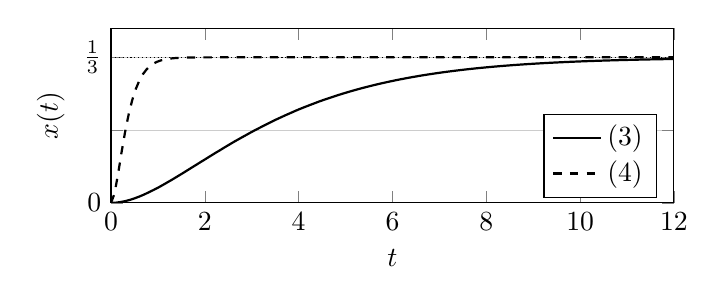
\begin{tikzpicture}
\begin{axis}[
  width=0.72\linewidth, height=3.8cm,
  xmin=0, xmax=12, ymin=0, ymax=0.4,
  xlabel={$t$}, ylabel={$x(t)$},
  ytick={0,0.1667,0.333}, yticklabels={$0$,,$\frac13$},
  ymajorgrids=true, grid style={gray!40}, legend pos=south east,
]
\addplot[thick,domain=0:12,samples=120]{1/3-2*exp(-0.5*x)+(5/3)*exp(-0.6*x)};
\addlegendentry{(3)}
\addplot[thick,dashed,domain=0:12,samples=160]{1/3-2*exp(-5*x)+(5/3)*exp(-6*x)};
\addlegendentry{(4)}
\addplot[densely dotted,domain=0:12]{1/3};
\end{axis}
\end{tikzpicture}
\end{center}

\subsection*{(4) $G_2(s)=\dfrac{1}{0.1s+1}$ の場合の比較}
同様に閉ループは
\begin{align*}
  &\qquad T(s)=\frac{1}{(s+1)(0.1s+1)+2}=\frac{1}{0.1s^2+1.1s+3}=\frac{10}{(s+5)(s+6)}.
\end{align*}
極は $s=-5,\ -6$、定常値 $T(0)=\dfrac13$。ステップ応答は
\[
  \therefore\quad \ans{\;x(t)=\dfrac13-2\e^{-5t}+\dfrac53\e^{-6t}\;}
\]
\textbf{考察}：両系とも定常値は $\dfrac13$ で等しい。違いは過渡特性に現れる。
\begin{itemize}\setlength{\itemsep}{1pt}
  \item \textbf{ゲイン線図}：$G_2$ の折れ点が $\omega=0.1\to10$ へ移り、$-20\,$dB/dec の帯が
        $\omega=1\!\sim\!10$ まで広がる。すなわち帯域が約 10 倍に拡大する。
  \item \textbf{時間応答}：閉ループ極が $-0.5,-0.6\to-5,-6$ へ移り、時定数が約 $\tfrac{1}{10}$ に
        短縮される。よって (4) は (3) よりおよそ 10 倍速く定常値 $\tfrac13$ に整定する。
\end{itemize}

\bigskip
\noindent 検算: (1) $L=2/((s+1)(10s+1))$、(3) $T=1/(10s^2+11s+3)$ 極 $\{-0.5,-0.6\}$ 定常 $\tfrac13$、
(4) $T=10/((s+5)(s+6))$ 極 $\{-5,-6\}$ 定常 $\tfrac13$ を SymPy で確認✓。

\end{document}
